%  Typ dokumentu - článek, prezentace aj.
\documentclass[english]{article}

%  Nastaví vstupní a výstupní kódování znaků (encoding) a lokalizace
\usepackage[T1]{fontenc}
\usepackage[utf8]{inputenc}
\usepackage[english,czech]{babel}
\usepackage{icomma}

%  Formát papíru a odsazení od jeho okrajů
\usepackage[letterpaper]{geometry}
\geometry{verbose,tmargin=1.5cm,bmargin=2cm,lmargin=2cm,rmargin=2cm}

%  Umožňuje pracovat s grafikou
\usepackage{graphicx}
\usepackage{bigstrut}
\usepackage{epstopdf}

%  Automaticky odsadí i první paragraf v každé sekci
\usepackage{indentfirst}

%  Umožňuje rozdělovat obsah na více sloupců
\usepackage{multicol}
\usepackage{booktabs}
\usepackage{pgffor}

%  Umožňuje používat hypertextové odkazy, nastavuje jejich barvu a vlastnosti
\usepackage[unicode]{hyperref}
\hypersetup{
	colorlinks=true, citecolor=blue, filecolor=blue, linkcolor=blue,
	urlcolor=blue
}

%  Umožnění odstranění italiky u jednotek
\newcommand{\unit}[1]{~\mathrm{#1}}
\newcommand{\unitb}[1]{~\mathrm{[#1]}}
\newcommand{\unitbr}[1]{\qquad\mathrm{[#1]}}

%  Formátování stránek, empty = odstraní číslování
% \pagestyle{empty}

%  Řádkování
\linespread{1.2}

%  Lepší zobrazování matematiky (rozšíření sum o \limits atd.)
%  Umožní psát přes \mathbb{N/R/Q/..} množiny čísel
\everymath{\displaystyle}
\usepackage{amsmath, amsthm, amssymb, wasysym}

%  Velikost fontu matematických výrazů v dokumentu lze pro danou
% základního fontu dokumentu upravit pomocí:
% \DeclareMathSizes{X}{Y}{Z}{U} kde:
% X je velikost fontu v dokumentu, pro kterou se matematika upraví
% Y je standartní velikost fontu matematiky
% Z je velikost fontu zmenšených (vnořených výrazů)
% U je velikost fontu ještě více zmenšených (vnořených výrazů).
\DeclareMathSizes{10}{10.5}{9}{9}

%  Nastaví autora, název, datum, skupinu měření apod. 
%  (můj vlastní příkaz, umožní znovu-použití v dokumentu)
\newcommand{\Author}{David Roesel}
\newcommand{\Coauthor}{Schönfeldová, Vyšín}
\newcommand{\Institute}{FJFI ČVUT v Praze}
\newcommand{\Subject}{VAKUOVÁ FYZIKA A TECHNIKA}
\newcommand{\Group}{Pá 14:30}
\newcommand{\Kruh}{FE}
\newcommand{\Title}{Úloha \#6  \\Vakuové napařování}
\newcommand{\Date}{12.12.2014}

% Custom comands
\newcommand{\dd}{\mathrm{d}}
\newcommand{\dln}{\mathrm{ln}}
\newcommand{\ee}{\mathrm{e}}
\newcommand{\degc}{^\circ C}
\newcommand{\jelina}{Oooo, Jelina!}

% Začátek dokumentu - Formátování na výstup
\begin{document}

% Interní proměnné, možno zobrazovat u prezentací, používají se při
% generování pomocí \titlepage apod.
\author{\Author}
\title{\Title}
\date{\Date}

%  Lokalizace některých názvů do češtiny
\renewcommand{\figurename}{Obr.}
\renewcommand{\tablename}{Tab.}
\renewcommand{\refname}{Reference}

% --- Hlavička dokumentu -----------------------------------------------

\setlength{\parindent}{0cm}
\begin{multicols}{2}
\textbf{\Subject \\
        \Institute \\[0.1cm]
%\large  \Title \\[0.5cm]
\Title \\[0.5cm]
}
\begin{tabular}{rlrl}
\large Datum měření: & \Date & \large Skupina: & \Group \\
\large Jméno: & \Author & \large Kroužek:  & \Kruh\\
\large Spolupracovali: & \Coauthor &\large Klasifikace:\\
\end{tabular}

\begin{flushright}

\includegraphics[scale=0.28]{../../_meta/fjfi_standart.pdf}
\hspace{0.2cm}
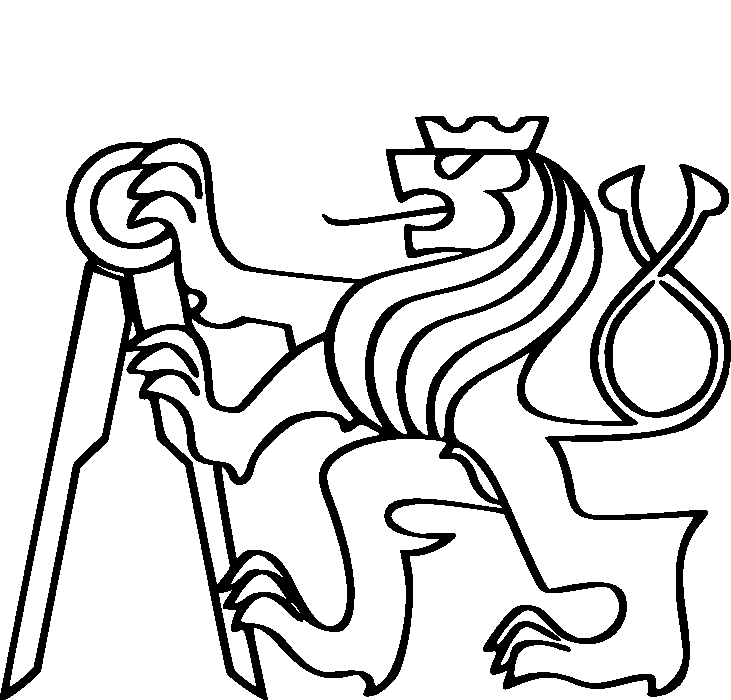
\includegraphics[scale=0.28]{../../_meta/cvut_standart.pdf}
\end{flushright}
\end{multicols}
\hrule
\vspace{0.5cm}

% ----------------------------------------------------------------------


% --- Tělo dokumentu ---------------------------------------------------
\setlength{\parindent}{0.5cm}

\section{Pracovní úkoly}

\begin{enumerate}
	\item Zapněte přívod el. napětí, vody a tlakového vzduchu a uveďte aparaturu AV 63 do provozu. Sledujte funkci aparatury a tlak až do cca $4\cdot 10^{-3}\unit{Pa}$.
	\item Připravte sklíčka na napařování a vložte je na stolek do aparatury. Připravte k napaření vrstvy cca 10~nm stříbra. Vložte drátek Ag do odpařovací vaničky. Uzavřete aparaturu zvonem a čerpejte do vysokého vakua $p < 5\cdot 10^{-3}\unit{Pa}$.
	\item Zvyšováním napětí regulačním trafem zvyšujte pomalu teplotu vaničky a pozorujte Ag drátek. Po dosažení teploty tání stříbra, až se drátek smrští do kuličky, odkryjte clonku a začněte napařovat.
	\item Vypněte žhavení a počkejte, až vanička zchladne. Poté napusťte recipient vzduchem a vyjměte napařené sklíčko.
	\item Postup opakujte se sklíčkem, na které otisknete palec.
\end{enumerate}

\section{Úvod}
	Ve všech dosavadních úlohách jsme zkoušeli, jak čerpat pomocí nejrůznějších vývěv, jak zefektivnit jejich čerpání, případně jak hledat netěsnosti pro zlepšení vakua. Všechny tyto znalosti se hodí například k napařování tenkých vrstev, které je důležitou aplikací vakuové techniky. Využívá se ve vědě i průmyslu, například pokud chceme tenkou vrstvu napařit na vzorek, který není vodivý, a my se na něj potřebujeme podívat v elektronovém mikroskopu s větším rozlišením. Principem metody je kondenzace par materiálu, který napařujeme, na podložce. V aparatuře je potřeba pro napařování udržovat nízký tlak, aby molekuly deponovaného materiálu byly schopné urazit dráhu k podložce, která pro úspěšné napařování musí být co nejčistší.

\section{Vypracování}
    \subsection{Teoretický úvod}
    	Pro napařování jsme používali vakuovou aparaturu AV 63 s rotační a difusní vývěvou. Všechny kroky, které jsme v předchozích úlohách dělali manuálně, jsme tentokrát nemuseli řešit, jelikož je obstaral programátor připojený k aparatuře. Schéma aparatury je na Obr.~\ref{fig:s_aparatura}, ačkoliv není příliš detailní a zobrazuje jen několik ventilů a použité vývěvy - detailnější schéma aparatury je vidět přímo na programátoru, který zároveň ukazuje, jaké části jsou a nejsou v provozu. Materiál, který napařujeme, je ohříván v odporově vyhřívané vaničce a její teplota je ovládána trafem ve spodní části aparatury. \newpage
    	
    		
    				\begin{figure}[h!]
    					\begin{center}
    						%\vspace*{-0.5cm}
    						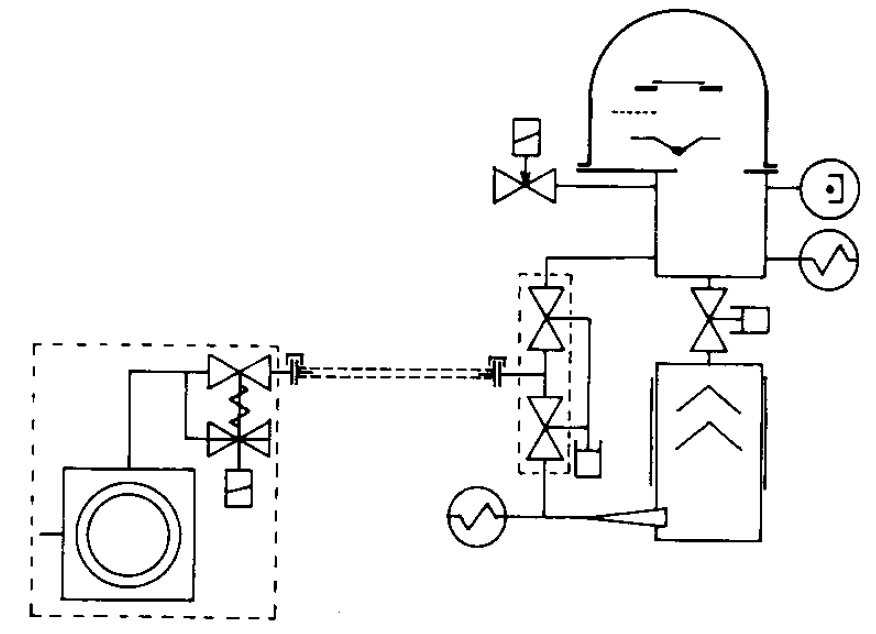
\includegraphics[width=0.55\linewidth]{../att/schema.png}
    						%\vspace*{-0,7cm}
    						\caption{Vakuové schema napařovací aparatury (převzato z \cite{bib:praskripta}). }
    						\label{fig:s_aparatura}
    					\end{center}
    				\end{figure}
    	
    	Stříbrný drátek, který používáme jako zdroj napařovaného stříbra, bylo třeba připravit správně dlouhý. Jeho průměr byl
    	\begin{equation}
    		d = 0,5\unit{mm}.
    	\end{equation}
    	Vzdálenost napařovacího sklíčka od vaničky se stříbrem byla
    	\begin{equation}
    		R = 125\unit{cm}
    	\end{equation}
    	a za úkol jsme měli napařit vrstvu o tloušťce
    	\begin{equation}
    		t = 10\unit{nm}.
    	\end{equation}
    	Pro určení potřebné délky stříbrného drátu jsme uvažovali, že objem stříbra ve vaničce musí být roven objemu 10nm vrstvy na myšlené polokouli o poloměru $R$. Výpočet jsme počítali příliš přesně vzhledem k charakteru úlohy jako
    	\begin{equation}
    		V_d = \frac{V_R - V_{R-t}}{2},
    	\end{equation}
    	kde $V_R$ je objem koule o poloměru $R$, $V_{R-t}$ objem koule o poloměru $R-t$ a $V_d$ potřebný objem drátku, pro který platí
    	\begin{equation}
    		V_d = \pi \left(\frac{d}{2}\right)^2\cdot l,
    	\end{equation} 
    	kde $l$ je hledaná délka drátu. Z tohoto vzorce za dosazení výše zmíněných hodnot dostáváme pro potřebnou délku stříbrného drátu výsledek
    	\begin{equation}
    		l = 5\unit{mm}.
    	\end{equation}

    \subsection{Postup měření}				
		Po příchodu k aparatuře jsme se s ní nejprve seznámili a detailně jsme prostudovali strany 27 a 28 z manuálu u úlohy, kde byl návod na režim vysokého vakua. Jako první jsme si nechali zapnout přívod tlakového vzduchu, chladící vody pro difusní vývěvu a elektrického napětí. 
		
		Následně jsme vypnuli všechna tlačítka na programátoru (pro vypnutí tlačítka \texttt{VENTING} bylo třeba jemně namáčknout tlačítko \texttt{PUMPING}). Poté jsme celý systém uvedli do provozu otočením hlavního spínače a stisknutím tlačítek \texttt{MAINS} na vakuometru a programátoru. Následně jsme stiskli tlačítko odpovídající režimu vysokého vakua a čekali, než dostatečně klesne tlak (přibližně 50 minut). K čerpání se využívala nejprve rotační vývěva, která čerpala difusní vývěvu, a poté i ta (po jejím dostatečném zahřátí). Po dosažení dostatečné teploty $\ge 200\unit{\degc}$ se automaticky otevíraly ventily tak, aby byl difusní či rotační vývěvou čerpán recipient (na aparaturu muselo být nandáno skleněné víko). 
	
		
		Zatímco aparatura čerpala na dostatečně nízký tlak, připravovali jsme si sklíčka na napaření. Ty jsme nejprve ručně očistili od velkých nečistot, poté jsme je dali do destilované vody s kapkou saponátu a nechali chvíli stát v ultrazvukové čističce. Nakonec jsme je opláchli destilovanou vodou a acetonem, přičemž zbytek acetonu jsme nechali odsát buničinou, na kterou jsme sklíčko bokem odložili. Dále jsme se sklíčkem pracovali výhradně pinzetou.
		
		Pro vlastní napařování jsme napustili krycí nádobu (\texttt{VENTING}) a sejmuli ji z aparatury. Pinzetou jsme sklíčko umístili pod jistící svorky na místo jemu určené a do vaničky jsme umístili dříve změřený a odříznutý kousek stříbrného drátu. Krycí nádobu jsme po otření jejího těsnění acetonem vrátili zpět a zahájili čerpání (tlačítkem \texttt{PUMPING}). Po odčerpání do tlaku okolo $5\cdot 10^{-3}\unit{Pa}$ jsme nbejprve odpařili nečistoty z drátku a následně zvyšovali napětí na regulačním transformátoru a sledovali stříbrný drátek. V momentu, kdy se z drátku stala kulička, jsme odkryli clonku a zahájili napařování. Vyčkali jsme, dokud stříbrná kulička nezmizela, a poté jsme nechali aparaturu vychladnout, napustili ji vzduchem a sklíčko vyndali. Totéž jsme opakovali pro druhé sklíčko po otisknutí palce na jeho napařovaný povrch. 
		
		Pro vypnutí aparatury stačilo zmáčknout tlačítko \texttt{STOP}, počkat, než se aparatura zchladí i za pomoci externího ventilátoru, který foukal vzduch na difusní vývěvu, a vypnout hlavní vypínač.
			
%	\subsection{Naměřené hodnoty}
					
	\subsection{Diskuse}
		Úspěšně jsme si vyzkoušeli, jak funguje aparatura na napařování. Sklíčko bez otisku prvku bylo lesklé a poloprůhledné. Objekty, které jsme skrze něj pozorovali, se nám jevily šedé a byly méně osvětlené. Na druhém sklíčku (s otiskem prstu) bylo patrné, že se v místech s mastnotou nezachytilo stříbro téměř vůbec, ačkoliv okolo otisku vypadalo stejně jako první sklíčko, což odpovídá předpokladu, že na mastných oblastech stříbro špatně drží. V obou případech stříbrná vrstva na skle velice špatně držela a dala se snadno setřít i letmým dotykem. To mohlo být způsobeno špatným očištěním sklíčka.
								
\section{Závěr}
	Nechali jsme zapnout přívod elektrického napětí, vody a tlakového vzduchu a uvedli jsme aparaturu $\mathrm{AV~63}$ do provozu. Sledovali jsme funkci aparatury a tlak až do cca $4\cdot 10^{-3}\unit{Pa}$. 
	
	Připravili jsme sklíčka na napařování a vložili jsme je na stolek do aparatury. Připravili jsme stříbro k napaření vrstvy cca 10~nm. Vložili jsme drátek $\mathrm{Ag}$ do odpařovací vaničky, uzavřeli jsme aparaturu zvonem a čerpali jsme do vysokého vakua $p\le 5 \cdot 10^{-3}\unit{Pa}$. 
	
	Pomalu jsme zahřívali vaničku za pozorování $\mathrm{Ag}$ drátku. Po dosažení teploty tání stříbra, když se drátek smrští do kuličky, jsme odkryli clonku a začali jsme napařovat.
	
	Postup jsme poté opakovali se sklíčkem, na které jsme otiskli palec.
	
	
\section {Použitá literatura}
% --- Literatura a reference -------------------------------------------
\begingroup
\renewcommand{\section}[2]{}

\begin{thebibliography}{9}

%\bibitem{bib:chyby} Kolektiv KF, \emph{Chyby měření} [Online], [cit. \today] \newline http://praktikum.fjfi.cvut.cz/documents/chybynav/chyby-o.pdf

\bibitem{bib:praskripta}Král, J.: \emph{Cvičení z vakuové techniky},
Vydavatelství ČVUT, Praha, 1996

%\bibitem{bib:tlak}ČHMÚ: \emph{Aktuální informace o počasí na území České republiky}, {[}online{]}, {[}cit. \today{]},\\ http://pr-asv.chmi.cz/synopy-map/pocasisp.php?ukazatel=stanice\&pozadi=\&pozadi=mapareg\&graf=ano

%\bibitem{bib:tabulky} J. Mikulčák a kol., Matematické, fyzikální a chemické tabulky \& vzorce. Prometheus,
%Praha 2009.\newline
%ISBN 978-80-7196-264-9

\end{thebibliography}
\endgroup
% ----------------------------------------------------------------------
\setcounter{equation}{0}
\numberwithin{equation}{section}

%\clearpage
%\part*{Přílohy}

%%%%\section{Domácí příprava}
%%%%	Domácí příprava je přiložena k protokolu.
%%%%\clearpage
%%%\section{Statistické zpracování dat}
%%%	Pro statistické zpracování využíváme aritmetického průměru:
%%%	\begin{equation} \label{eq:aritmeticky_prumer}
%%%	\overline{x} = \frac{1}{n}\sum\limits_{i=1}^{n}x_i,
%%%	\end{equation}
%%%
%%%%	jehož směrodatnou odchylku spočítáme jako 
%%%%	\begin{equation} \label{eq:smodch_aritmetickeho_prumeru}
%%%%	\sigma_0 = \sqrt{\frac{1}{n} \sum\limits_{i=1}^{n}\left( x_i - \overline{x} \right)^2 },
%%%%	\end{equation}
%%%%	
%%%%	kde $ x_i $ jsou jednotlivé naměřené hodnoty, $ n $ je počet měření, $ \overline{x} $ aritmetický průměr a $ \sigma_0 $ jeho chyba \cite{bib:chyby}.
%%%	
%%%	
%%%	jehož chybu spočítáme jako 
%%%	\begin{equation} \label{eq:chyba_aritmetickeho_prumeru}
%%%	\sigma_0 = \sqrt{\frac{1}{n(n-1)} \sum\limits_{i=1}^{n}\left( x_i - \overline{x} \right)^2 },
%%%	\end{equation}
%%%	
%%%	kde $ x_i $ jsou jednotlivé naměřené hodnoty, $ n $ je počet měření, $ \overline{x} $ aritmetický průměr a $ \sigma_0 $ jeho chyba \cite{bib:chyby}.
%%%%	
%%%Při nepřímém měření počítáme hodnotu s chybou dle následujících vztahů:
%%%	\begin{equation}
%%%	u = f(x, y, z, \ldots),
%%%	\end{equation}
%%%	\begin{displaymath}
%%%	x = (\overline{x} \pm \sigma_x), \qquad
%%%	y = (\overline{y} \pm \sigma_y), \qquad
%%%	z = (\overline{z} \pm \sigma_z), \qquad
%%%	\ldots,
%%%	\end{displaymath}
%%%	
%%%	kde $ u $ je veličina, kterou určujeme nepřímo z měřených veličin $ x, y, z, \ldots $ 
%%%	
%%%	Pak
%%%	\begin{displaymath}
%%%	\overline{u} = f(\overline{x}, \overline{y}, \overline{z}, \ldots),
%%%	\end{displaymath}
%%%	\begin{equation}\label{eq:chyba_neprime_mereni}
%%%	\sigma_u = \sqrt{\left( \frac{\partial f}{\partial x} \right)^2 \sigma^2_x + \left( \frac{\partial f}{\partial y} \right)^2 \sigma^2_y + \left( \frac{\partial f}{\partial z} \right)^2 \sigma^2_z + \ldots},
%%%	\end{equation}
%%%	\begin{displaymath}
%%%	u = (\overline{u} \pm \sigma_ u).
%%%	\end{displaymath}
%%	
%V případě, že máme několik různě přesných měření stejné veličiny, používáme vztah pro vážený průměr:
%	\begin{equation} 
%	\overline{x}=\frac{\sum\limits_{i=1}^{n}p_{i}x_{i}}{\sum\limits_{i=1}^{n}p_{i}},
%	\end{equation}
%	
%	kde $\overline{x}$ je vážený průměr, $x_{i}$ jsou jednotlivá měření a pro $p_{i}$ platí
%	 
%	\begin{equation}
%	p_{i}=\frac{1}{\sigma_{i}^{2}},
%	\end{equation}
%	
%	kde $\sigma_{i}$ jsou jednotlivé chyby daných měření.
%	 
%	Celkovou chybu tedy vypočítáme ze vztahu
%	\begin{equation} \label{eq:vazeny_prumer}
%	\sigma_{0}=\sqrt{\frac{1}{\sum\limits_{i=1}^{n}p_{i}}}.
%	\end{equation}
%
%\subsubsection{Metoda nejmenších čtverců}
%Snažíme-li se metodou nejmenších čtverců proložit data lineární závislostí $Y_i = ax_i+b$, dosazujeme hodnoty $x_i, y_i$ a snažíme se najít parametry $a$ a $b$ tak, aby byl součet všech kvadratických odchylek $\Delta Y_i^2$ minimální. Toho dosáhneme pomocí následujících vzorců \cite{bib:ctverce} :
%\begin{equation}\label{eq:ctverce_a}
%		a = \frac{n\sum\limits_{i=1}^{n}{x_i y_i}  - \sum\limits_{i=1}^{n}{x_i}\sum\limits_{i=1}^{n}{y_i}}{n\sum\limits_{i=1}^{n}{x_i^2}  - \left(\sum\limits_{i=1}^{n}{x_i}\right)^2}, \qquad \qquad
%		\sigma_a = \sqrt{\frac{n\sum\limits_{i=1}^{n}{(y_i - Y_i)^2} }{(n-2)\left(\sum\limits_{i=1}^{n}{x_i^2}  - \left(\sum\limits_{i=1}^{n}{x_i}\right)^2\right)}},
%\end{equation}
%
%\begin{equation}\label{eq:ctverce_b}
%		b = \frac{\sum\limits_{i=1}^{n}{x_i^2} \sum\limits_{i=1}^{n}{y_i}  - \sum\limits_{i=1}^{n}{x_i}\sum\limits_{i=1}^{n}{x_i y_i}}{n\sum\limits_{i=1}^{n}{x_i^2}  - \left(\sum\limits_{i=1}^{n}{x_i}\right)^2}, \qquad \qquad
%		\sigma_b = \sqrt{\frac{\sum\limits_{i=1}^{n}{x_i^2}\sum\limits_{i=1}^{n}{(y_i - Y_i)^2} }{n(n-2)\left(\sum\limits_{i=1}^{n}{x_i^2}  - \left(\sum\limits_{i=1}^{n}{x_i}\right)^2\right)}}.
%\end{equation}
%\clearpage
	
%\clearpage
%\subsection{Tabulky a grafy}

%\clearpage
%\subsection{Schémata}
%	
%	\begin{figure}[h!]
%	\centering
%			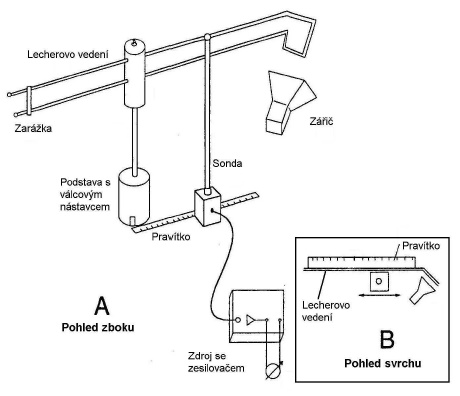
\includegraphics[width=13cm]{att/lecherovo_vedeni.jpg}
%			\caption{Experiment s Lecherovým vedením (převzato z  \cite{bib:zadani}). }
%			\label{fig:lecherovo_vlneni}
%	\end{figure}	
%	
%\clearpage
% --- Konec dokumentu --------------------------------------------------

\end{document}

